\subsection{Time interval selection}
Before selecting the best time interval we need to set two parameters: the threshold number of words in one \texttt{WindowOperation} and the threshold number of valid \texttt{WindowOperation} groups in one \texttt{Pad} (see Section \ref{sub:time_interval}). We set the minimum number of words to 10 according to the average length datasets STS2014-Forum (10.12 words), SICK2014 (9.67 words) \cite{sen2vec}. Also, in order to fit the similarity distribution we need enough similarity values in one \texttt{Pad}, so we set 5 as the minimum value of valid \texttt{WindowOperation} groups in a valid \texttt{Pad}. 
As we can see in Figure \ref{TimeInterval}, the candidate time intervals are from 60s to 380s. We chose 180s as it is the time interval with the most valid \texttt{Pads}.
\begin{figure}[htp]
    \centering
    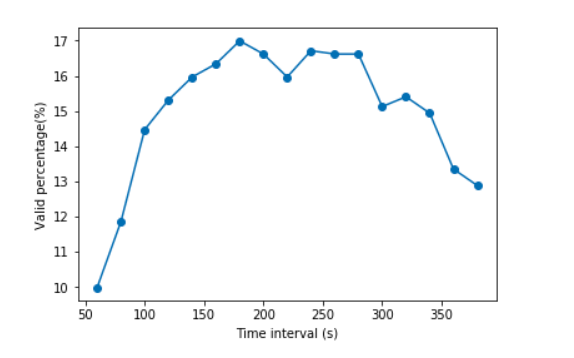
\includegraphics[width=0.5\textwidth]{figures/select_time_interval.png}
    \caption{Valid \texttt{Pad} percentage for different time interval durations}
    \label{TimeInterval}
\end{figure}

\subsection{Heuristics Analysis}
    We first look at the effect of considering only Operations after a specific start timestamp for computing \texttt{Pad} heuristics and compare it  to the score that considers \texttt{Operations} from the start. Then we see how \texttt{Paragraph} number and \texttt{Superparagraph} length evolve in time and we use time series analysis to see whether we could use these metrics to predict how much longer the students will take to finish the task.
    \subsubsection{Comparison between full Pad and window scores}
        We presented the need for modifying the scores that we were computing in the previous version of the tool so that the changes introduced by new \texttt{Operations} have a more noticeable impact.
        However, we need to keep in mind that some \texttt{Operations} may not be considered when using the window-contained Operations approach, particularly if some \texttt{Operations} are not fully contained within a single time window.

        Figures \ref{fig:typeoverallscorewrite} and \ref{fig:windowtypeoverallscorewrite} show the overall scores for writing operations, both using the defined time interval of 3 minutes. These Figures show in gray the boxplots of the score values per window for all pads, and in blue the average value with the standard deviation error bars.
    
        \begin{figure}[htp!]
            \centering
            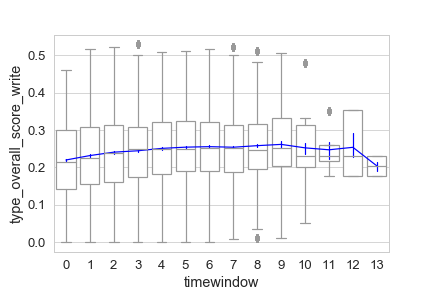
\includegraphics[width=0.5\textwidth]{figures/typeoverallscorewrite.png}
            \caption{Overall score for write type using 3 min time windows and considering Operations from the beginning of the Pad.}
            \label{fig:typeoverallscorewrite}
        \end{figure}
        \begin{figure}[htp!]
            \centering
            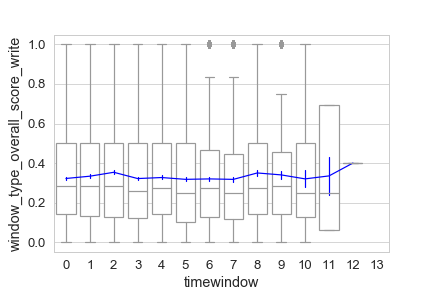
\includegraphics[width=0.5\textwidth]{figures/windowtypeoverallscorewrite.png}
            \caption{Overall score for write type using 3 min time windows and considering Operations from the beginning of the window (new implementation).}
            \label{fig:windowtypeoverallscorewrite}
        \end{figure}
        
        In Figure \ref{fig:typeoverallscorewrite} the line is smoother, as we are considering all the Operations from the beginning of the Pad until the end of the current window and therefore at every window we are averaging any possible changes with the rest of the Pad. Figure \ref{fig:windowtypeoverallscorewrite} shows the score changes from one window to another more clearly, as it is only considering the Operations within the time window. 
        
    \subsubsection{Paragraph and Superparagraph length in time} 
    In this section we decided to look at the number of paragraphs per superparagraph and at the average paragraph length and how these metrics change in time. We decided to try a simple model to see how well it could fit our data, and the results are shown in Figures \ref{fig:avg_p_sp} and \ref{fig:avg_len_p}. In both cases we decided to fit the values observed that correspond to windows 0 to 13, as windows 14 to 17 have less observations (because most paragraphs last 45 minutes or less, i.e. they last only 15 timewindows). However, we plot the results for windows 15 to 17 as well.
    
        \begin{figure}[htp!]
            \centering
            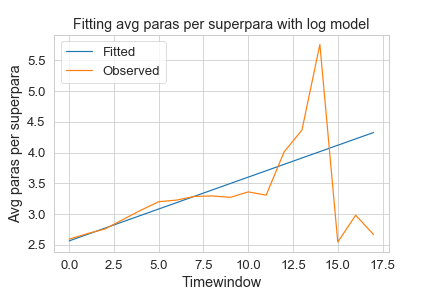
\includegraphics[width=0.5\textwidth]{figures/avg_p_sp.png}
            \caption{Average number of Paragraphs per Superparagraph. The linear model fitted has slope 0.1 and offset 2.55.}
            \label{fig:avg_p_sp}
        \end{figure}
        \begin{figure}[htp!]
            \centering
            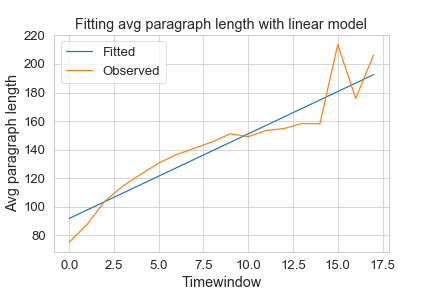
\includegraphics[width=0.5\textwidth]{figures/avg_len_p.png}
            \caption{Average length in characters per Paragraph. The linear model fitted has slope 5.9 and offset 91.8.}
            \label{fig:avg_len_p}
        \end{figure}
    
    From the two metrics obtained here we could obtain the value of the average Superparagraph length, as it would be the product of both.
    
    We see that the tendency does not seem to converge, so from these results we would not be able to say whether we could predict when the task will be finished. However, we need to keep in mind that the average for first windows has been computed over more pads than for the last windows. As we can see, up until timewindow 11 (which would correspond to minute 33 of the task), it seems like the values would converge. For this reason, it may be interesting to repeat this analysis after implementing a different WindowOperation split that takes into account the total duration of the pad.
\subsection{Semantic Analysis}
\label{sub:result_semantic}
Figure \ref{similar} shows the similarity value of three datasets. As we can see from those similarity values of each models for different similarity paragraph texts. \texttt{doc2vec} models can clearly recognize different similarity paragraph texts, but it has lower values even the the paragraph looks very similar and took the longest time to compute similarity. As for the fastest \texttt{spacy} model, it performed bad since the values of them are always very high even the two texts are totally different. And \texttt{sent2vec} model can correctly recognize them . Additionally, we can discover the different performances of those models when applying to same paragraph pair. \texttt{Spacy} model always have the highest values and  \texttt{doc2vec} always have the lowest values.  Overall, for each two paragraph pairs, the similarity difference(increase or decrease) between these two pairs are almost the same between different models. We finally chose \texttt{sent2vec} as our pre-trained model since it took less time and performed well in different similarity datasets.
    \begin{figure}[htp]
        \centering
        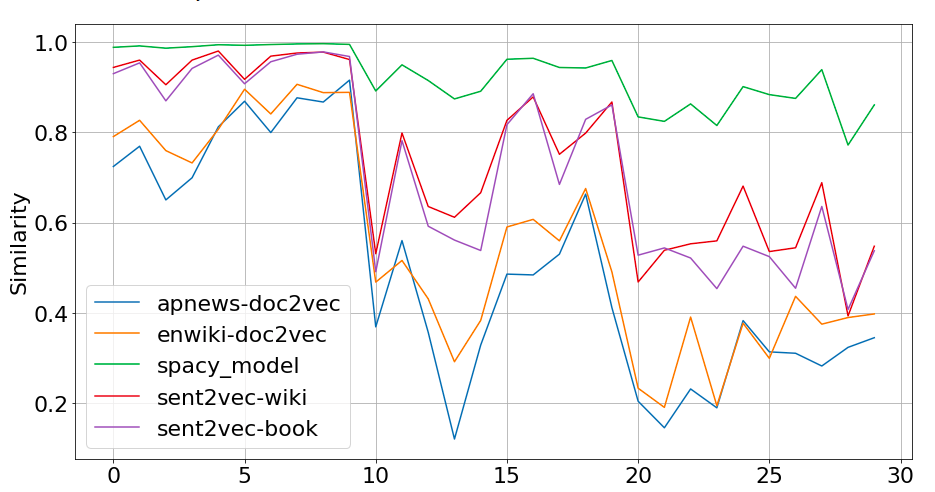
\includegraphics[width=0.5\textwidth]{figures/pre-trained-text.png}
        \caption{The evaluation similarity value of datasets}
        \label{similar}
    \end{figure}
    
\subsection{Fitting similarity distribution}
We could roughly separate our dataset into three categories depending on the trend of the semantic similarity distribution (increasing, stable and decreasing). However, at this point it is difficult to tell whether this classification would give us useful insights on the collaborative behavior  of the students.

Figure \ref{fitting} shows the similarity distribution of one valid \texttt{Pad}. We fitted a linear model to the observed data. From the Figure, we can easily see an increasing trend in topic similarity between this \texttt{Pad}'s authors, reflected in the positive slope of the fitted model. 

\begin{figure}[htp]
    \centering
    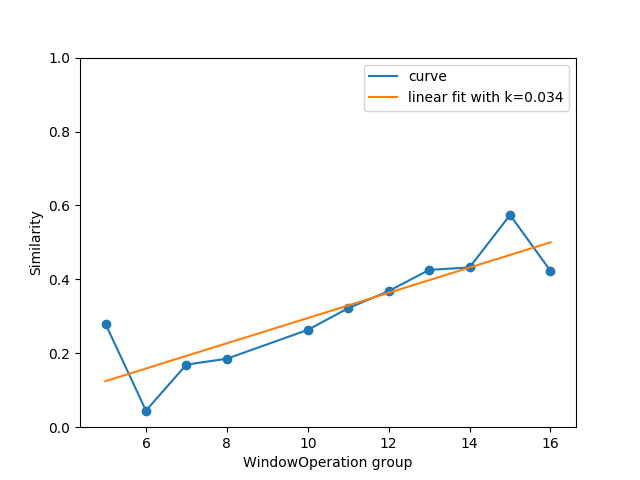
\includegraphics[width=0.5\textwidth]{figures/linear_fiting.png}
    \caption{Fitting similarity distribution}
    \label{fitting}
\end{figure}



\subsection{SuperParagraph similarity visualization}
When applying semantic analysis on \texttt{SuperParagraphs}, we first plot the heatmap for similarity values between all \texttt{SuperParagraphs} to get an overview of the document semantics. The heatmap in Figure \ref{similarity_heatmap} shows the inter \texttt{SuperParagraphs}' similarity in one document from our dataset.

We can conclude that \texttt{SuperParagraphs} 0 and 13 are the most different pair and \texttt{SuperParagraphs} 1 and 12 are the most similar pair. We include below the texts of those 4 \texttt{SuperParagraphs}, as it can be used to verify if we agree with the results and to get some intuition on how the results are computed:

\begin{figure}[htp]
    \centering
    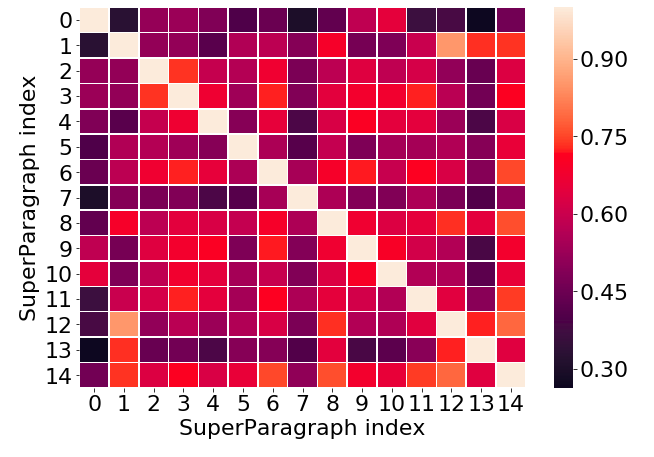
\includegraphics[width=0.49
    \textwidth]{figures/similarity_heatmap.png}
    \caption{Inter \texttt{SuperParagraph} similarity heatmap}
    \label{similarity_heatmap}
\end{figure}

\texttt{SuperParagraph 0}:\\
\textit{Your task is to act as an advisor to an official within the science  ministry. You are advising an official on the issues below. 
The official  is not an expert in the area, but you can assume they are a generally  informed reader.\\
They are interested in the best supported claims in the  documents. Produce a summary of the best supported claims you find and explain why you think they are.\\
Note you are not being asked to "create your own argument" or  "summarise everything you find" but rather, make a judgement about which  claims have the strongest support.}

\texttt{SuperParagraph 13}:\\
\textit{CONCLUSION:\\
Currently, glyphosate dominates crop weed control in soybean, maize,  canola and cotton in North and South America. Consequently, throughout  large areas, glyphosate reliance without diversity in weed control  practices is a strong selection pressure favoring the evolution and  eventual domination of glyphosate-resistant weed populations.}
\newpage
\texttt{SuperParagraph 1}:\\
\textit{INTRODUCTION :\\
Glyphosate  is the active ingredient in Roundup agricultural herbicides and other  herbicide formulations that are widely used for agricultural, forestry,  and residential weed control.\\
It is one of the most widely-used weedkillers in the  world, used by farmers, local government and gardeners, as well as  sprayed\\
extensively on some genetically modified crops imported into  Europe for use as animal feed.\\
Glyphosate,  N-(phosphonomethyl)glycine, is the most extensively used herbicide in  the history of agriculture. Weed management programs in glyphosate  resistant (GR) field crops have provided highly effective weed control,  simplified management decisions, and given cleaner harvested products}

\texttt{SuperParagraph 12}:\\
\textit{6.Glyphosate effects on diseases of plants\\
Glyphosate, N-(phosphonomethyl)glycine, is the most extensively used  herbicide in the history of agriculture. Weed management programs in  glyphosate resistant (GR) field crops have provided highly effective  weed control, simplified management decisions, and given cleaner  harvested products. However, this relatively simple, broad-spectrum,  systemic herbicide can have extensive unintended effects on nutrient  efficiency and disease severity, thereby threatening its agricultural sustainability.  Given that  recommended doses of glyphosate are often many times higher than needed  to control weeds, we believe the most prudent method to reduce the  detrimental effects of glyphosate on GR crops will be to use this  herbicide in as small a dose as practically needed. Such a frugal  approach will not only curtail disease predisposition of GR crops, but  will also benefit the grower and the 
environment.}

We also plotted the time evaluation of inter \texttt{Superparagraph} similarity. In Figure \ref{para_similarity}, each picture shows the evolution in time of the similarity between one \texttt{SuperParagraph} and all \texttt{SuperParagraphs}. The zero values at the beginning indicate that this \texttt{SuperParagraph} was not created yet.

\begin{figure}[htp]
    \centering
    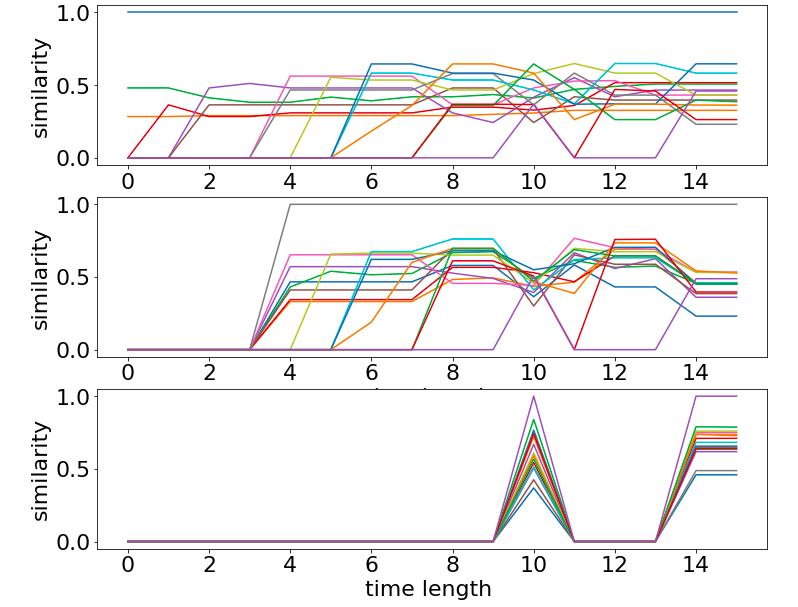
\includegraphics[width=0.49\textwidth]{figures/para_similarity.png}
    \caption{Inter \texttt{SuperParagraph} Similarity through time}
    \label{para_similarity}
\end{figure}

